\documentclass{beamer}
\usepackage{tikz}
\usepackage{fancyvrb}
\usepackage{xcolor}
\title{Intro To Asymmetric Cryptography\\RPISEC}
\date{October 29, 2019}
\author{Avi Weinstock (\Verb|aweinstock|)}

\setbeamercolor{normal text}{fg=white}
\setbeamercolor{frametitle}{fg=cyan}
\setbeamercolor{title}{fg=cyan}

%151820
%>>> [0x15,0x18,0x20]
%[21, 24, 32]
% convert rpisec_background.png -alpha set -fill '#15182080' -draw 'rectangle 0 0 1090 1216' rpisec_background2.png
% convert probable_prime.png -alpha set -fill '#15182080' -draw 'rectangle 0 0 414 836' probable_prime2.png
\definecolor{rpisecbgcolor}{RGB}{21, 24, 32}
\usebackgroundtemplate{
\colorbox{rpisecbgcolor}{\raisebox{1pt}[\paperheight][\depth]{\hspace{0.6\paperwidth}
%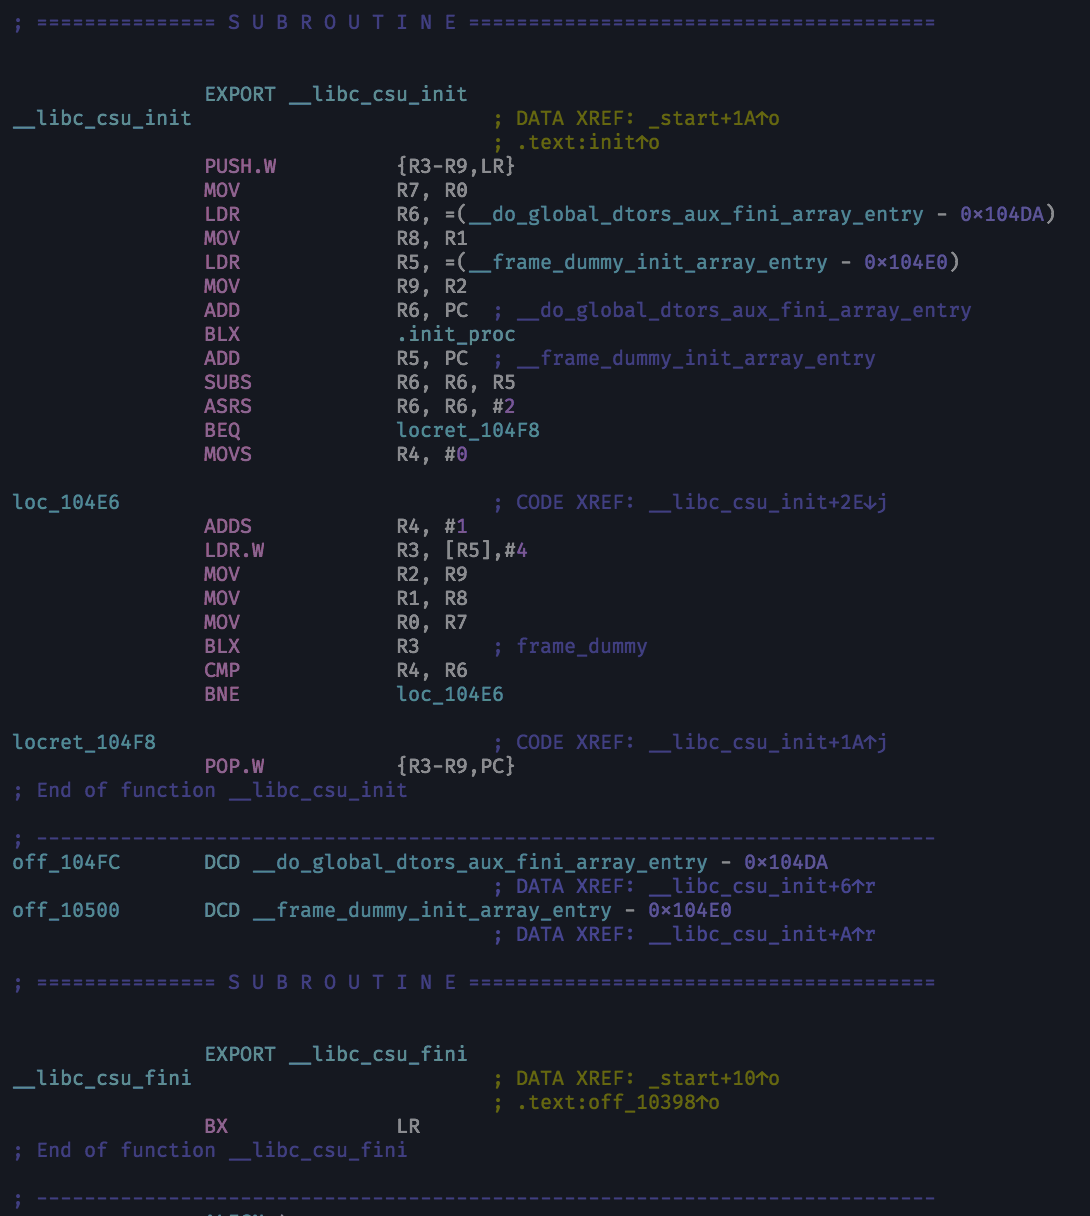
\includegraphics[width=0.4\paperwidth, height=\paperheight]{rpisec_background2.png}
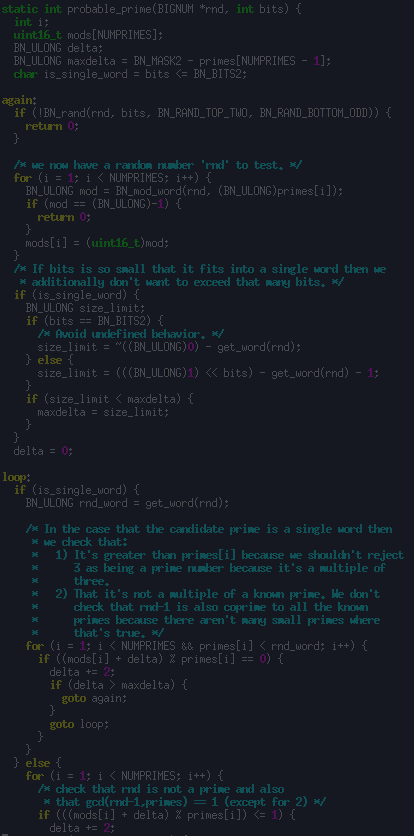
\includegraphics[width=0.4\paperwidth, height=\paperheight]{probable_prime2.png}
}}
}

\begin{document}
\maketitle

%\begin{frame}[fragile]
%\frametitle{Setup}
%\begin{itemize}
%\item Python libraries: \verb|pip install gmpy pycrypto pwntools|
%\item
%\verb|pycrypto| and \verb|gmpy| practically required, \verb|pwntools| is merely recommended.
%\end{itemize}
%\end{frame}

\begin{frame}[fragile]
\frametitle{Symmetric vs Asymmetric Cryptosystems}
\begin{minipage}[t]{0.45\textwidth}
Examples of symmetric crypto:
\begin{itemize}
\item classical ciphers (caesar, vigenere)
\item block ciphers (DES, AES)
\item stream ciphers (OTP, RC4, Salsa20)
\item hash functions (MD5, SHA256)
\item MACs (HMAC, Poly1305)
\end{itemize}
\end{minipage}
\begin{minipage}[t]{0.5\textwidth}
Examples of asymmetric crypto:
\begin{itemize}
\item key exchange (Diffie-Hellman)
\item encryption (RSA, ElGamal)
\item signatures (RSA, DSA, Schnorr)
\item homomorphic encryption (Paillier, RSA, Gentry)
\end{itemize}
\end{minipage}
\end{frame}

\begin{frame}[fragile]
\frametitle{What is the significance of RSA?}
\begin{itemize}
\item Historically the first asymmetric cryptosystem (published in 1977)
\item Named for its inventors: Rivest, Shamir, Adleman
\item Very flexible: can be used for both encryption and signing, is multiplicatively homomorphic
\item Easy to implement
\item Easy to mess up implementing, on account of its flexibility
\end{itemize}
\end{frame}

\begin{frame}[fragile]
\frametitle{What is RSA?}
\begin{itemize}
\item $p$ and $q$ are distinct large primes
\item $n = p * q$
\item $\varphi(n) = (p-1)*(q-1)$
\item $e * d \equiv 1\hspace{1mm}(\text{mod } \varphi(n))$
\item $(n, e)$ is the "public key"
\item $(p, q, d)$ is the "private key"
\item $\verb|enc|(x) = \verb|rem|(x^e, n)$
\item $\verb|dec|(x) = \verb|rem|(x^d, n)$
\end{itemize}
\end{frame}

\begin{frame}[fragile]
\frametitle{Euclidean division}
\begin{minipage}{0.4\textwidth}
% convert diagrams/euclidean_division.png -negate diagrams/euclidean_division_negated.png

\includegraphics[width=0.9\textwidth]{diagrams/euclidean_division_negated.png}\\
\end{minipage}
\begin{minipage}{0.5\textwidth}
\begin{itemize}
\item $\forall x, y \exists q, r (y*q + r = x)$
\item $q = \verb|quot|(x, y)$
\item $r = \verb|rem|(x, y)$
\item $0 \le r < y$
\item $3 * 27 + 1 = 82$
\end{itemize}
\end{minipage}
\end{frame}

\begin{frame}[fragile]
\frametitle{Modular congruence and primes}
Divides cleanly/Is divisor of:
\begin{itemize}
\item $\verb|divides|(x, y) \leftrightarrow \verb|rem|(y, x) = 0$
\item e.g. $\verb|divides|(5, 10)$, since \verb|10 % 5 == 0|
\end{itemize}
Modular congruence:
\begin{itemize}
\item $x \equiv y\hspace{1mm}(\text{mod } n) \leftrightarrow \verb|divides|(x-y, n)$
\item $x \equiv y\hspace{1mm}(\text{mod } n) \leftrightarrow \verb|rem|(x, n) = \verb|rem|(y, n)$
\end{itemize}
Primeness:
\begin{itemize}
\item $\verb|prime|(p) \leftrightarrow \forall k \in [2, p-1](\neg\verb|divides|(k, p))$
\item \begin{Verbatim}[fontsize=\tiny]
def prime(p):
    return all([p % k != 0 for k in range(2,p)])

assert filter(prime, range(2, 20)) == [2, 3, 5, 7, 11, 13, 17, 19]
\end{Verbatim}
\end{itemize}
Greatest Common Divisor:
\begin{itemize}
\item $\verb|gcd|(x, y) = \text{max}\{ k | \verb|divides|(k, x) \land \verb|divides|(k, y)\}$
\item \begin{Verbatim}[fontsize=\tiny]
def gcd(x, y):
    return max([1]+[k for k in range(1, x*y) if x % k == 0 and y % k == 0])
\end{Verbatim}
%>>> def gcd(x, y):
%...     return max([1]+[k for k in range(1, x*y) if x % k == 0 and y % k == 0])
%...
%>>> [[[(a,b) for (a,b) in [(gmpy.gcd(x, y),gcd(x,y))] if a != b] for x in range(1, 100)] for y in range(1, 100)]
\end{itemize}
\end{frame}

\begin{frame}[fragile]
\frametitle{Modular arithmetic}
\begin{itemize}
\item Let $\mathbb Z_n$ denote $\{ \verb|rem|(x, n) | x \in \mathbb Z \}$, or equivalently, $[0, n)$.
\item We can truncate addition and multiplication to work within $\mathbb Z_n$ by calculating remainders after each operation
\item {\scriptsize "Clock arithmetic": in $\mathbb Z_{12}$, $9 + 4 = 1$, since $\verb|rem|(9+4, 12) = \verb|rem|(13, 12) = 1$}
\end{itemize}
% wget https://upload.wikimedia.org/wikipedia/commons/thumb/a/a4/Clock_group.svg/560px-Clock_group.svg.png -O diagrams/560px-Clock_group.png
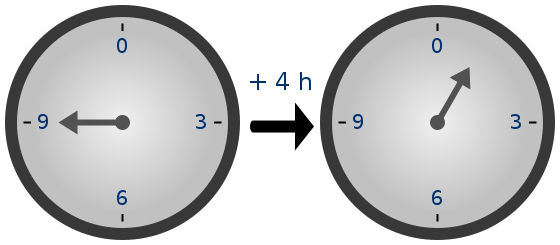
\includegraphics[width=0.9\textwidth]{diagrams/560px-Clock_group.png}\\
\end{frame}

\begin{frame}[fragile]
\frametitle{Addition and Multiplication mod 7}
\(\begin{array}{p{3mm}|p{2mm}p{2mm}p{2mm}p{2mm}p{2mm}p{2mm}p{2mm}}
\(+\) & 0 & 1 & 2 & 3 & 4 & 5 & 6\\\hline
0 & 0 & 1 & 2 & 3 & 4 & 5 & 6\\
1 & 1 & 2 & 3 & 4 & 5 & 6 & 0\\
2 & 2 & 3 & 4 & 5 & 6 & 0 & 1\\
3 & 3 & 4 & 5 & 6 & 0 & 1 & 2\\
4 & 4 & 5 & 6 & 0 & 1 & 2 & 3\\
5 & 5 & 6 & 0 & 1 & 2 & 3 & 4\\
6 & 6 & 0 & 1 & 2 & 3 & 4 & 5\\
\end{array}\)\hspace{0.5cm}\(\begin{array}{p{3mm}|p{2mm}p{2mm}p{2mm}p{2mm}p{2mm}p{2mm}p{2mm}}
\(*\) & {\color{cyan}0} & {\bf\color{green}1} & {\color{white}2} & {\color{white}3} & {\color{white}4} & {\color{white}5} & {\color{white}6}\\\hline
{\color{cyan}0}&{\color{cyan}0}&{\color{cyan}0}&{\color{cyan}0}&{\color{cyan}0}&{\color{cyan}0}&{\color{cyan}0}&{\color{cyan}0}\\
{\bf\color{green}1}&{\color{cyan}0}&{\bf\color{green}1}&{\color{white}2}&{\color{white}3}&{\color{white}4}&{\color{white}5}&{\color{white}6}\\
{\color{white}2}&{\color{cyan}0}&{\color{white}2}&{\color{white}4}&{\color{white}6}&{\bf\color{green}1}&{\color{white}3}&{\color{white}5}\\
{\color{white}3}&{\color{cyan}0}&{\color{white}3}&{\color{white}6}&{\color{white}2}&{\color{white}5}&{\bf\color{green}1}&{\color{white}4}\\
{\color{white}4}&{\color{cyan}0}&{\color{white}4}&{\bf\color{green}1}&{\color{white}5}&{\color{white}2}&{\color{white}6}&{\color{white}3}\\
{\color{white}5}&{\color{cyan}0}&{\color{white}5}&{\color{white}3}&{\bf\color{green}1}&{\color{white}6}&{\color{white}4}&{\color{white}2}\\
{\color{white}6}&{\color{cyan}0}&{\color{white}6}&{\color{white}5}&{\color{white}4}&{\color{white}3}&{\color{white}2}&{\bf\color{green}1}\\
\end{array}\)
\end{frame}

\begin{frame}[fragile]
\frametitle{Addition and Multiplication mod 8}
\(\begin{array}{p{3mm}|p{2mm}p{2mm}p{2mm}p{2mm}p{2mm}p{2mm}p{2mm}p{2mm}}
\(+\) & {\color{cyan}0} & {\bf\color{green}1} & {\color{white}2} & {\color{white}3} & {\color{white}4} & {\color{white}5} & {\color{white}6} & {\color{white}7}\\\hline
{\color{cyan}0}&{\color{cyan}0}&{\bf\color{green}1}&{\color{white}2}&{\color{white}3}&{\color{white}4}&{\color{white}5}&{\color{white}6}&{\color{white}7}\\
{\bf\color{green}1}&{\bf\color{green}1}&{\color{white}2}&{\color{white}3}&{\color{white}4}&{\color{white}5}&{\color{white}6}&{\color{white}7}&{\color{cyan}0}\\
{\color{white}2}&{\color{white}2}&{\color{white}3}&{\color{white}4}&{\color{white}5}&{\color{white}6}&{\color{white}7}&{\color{cyan}0}&{\bf\color{green}1}\\
{\color{white}3}&{\color{white}3}&{\color{white}4}&{\color{white}5}&{\color{white}6}&{\color{white}7}&{\color{cyan}0}&{\bf\color{green}1}&{\color{white}2}\\
{\color{white}4}&{\color{white}4}&{\color{white}5}&{\color{white}6}&{\color{white}7}&{\color{cyan}0}&{\bf\color{green}1}&{\color{white}2}&{\color{white}3}\\
{\color{white}5}&{\color{white}5}&{\color{white}6}&{\color{white}7}&{\color{cyan}0}&{\bf\color{green}1}&{\color{white}2}&{\color{white}3}&{\color{white}4}\\
{\color{white}6}&{\color{white}6}&{\color{white}7}&{\color{cyan}0}&{\bf\color{green}1}&{\color{white}2}&{\color{white}3}&{\color{white}4}&{\color{white}5}\\
{\color{white}7}&{\color{white}7}&{\color{cyan}0}&{\bf\color{green}1}&{\color{white}2}&{\color{white}3}&{\color{white}4}&{\color{white}5}&{\color{white}6}\\
\end{array}\)\hspace{0.5cm}\(\begin{array}{p{3mm}|p{2mm}p{2mm}p{2mm}p{2mm}p{2mm}p{2mm}p{2mm}p{2mm}}
\(*\) & {\color{cyan}0} & {\bf\color{green}1} & {\color{white}2} & {\color{white}3} & {\color{white}4} & {\color{white}5} & {\color{white}6} & {\color{white}7}\\\hline
{\color{cyan}0}&{\color{cyan}0}&{\color{cyan}0}&{\color{cyan}0}&{\color{cyan}0}&{\color{cyan}0}&{\color{cyan}0}&{\color{cyan}0}&{\color{cyan}0}\\
{\bf\color{green}1}&{\color{cyan}0}&{\bf\color{green}1}&{\color{white}2}&{\color{white}3}&{\color{white}4}&{\color{white}5}&{\color{white}6}&{\color{white}7}\\
{\color{white}2}&{\color{cyan}0}&{\color{white}2}&{\color{white}4}&{\color{white}6}&{\color{cyan}0}&{\color{white}2}&{\color{white}4}&{\color{white}6}\\
{\color{white}3}&{\color{cyan}0}&{\color{white}3}&{\color{white}6}&{\bf\color{green}1}&{\color{white}4}&{\color{white}7}&{\color{white}2}&{\color{white}5}\\
{\color{white}4}&{\color{cyan}0}&{\color{white}4}&{\color{cyan}0}&{\color{white}4}&{\color{cyan}0}&{\color{white}4}&{\color{cyan}0}&{\color{white}4}\\
{\color{white}5}&{\color{cyan}0}&{\color{white}5}&{\color{white}2}&{\color{white}7}&{\color{white}4}&{\bf\color{green}1}&{\color{white}6}&{\color{white}3}\\
{\color{white}6}&{\color{cyan}0}&{\color{white}6}&{\color{white}4}&{\color{white}2}&{\color{cyan}0}&{\color{white}6}&{\color{white}4}&{\color{white}2}\\
{\color{white}7}&{\color{cyan}0}&{\color{white}7}&{\color{white}6}&{\color{white}5}&{\color{white}4}&{\color{white}3}&{\color{white}2}&{\bf\color{green}1}\\
\end{array}\)
\end{frame}

\begin{frame}[fragile]
\frametitle{Multiplicative inverses}
\begin{itemize}
\item In $\mathbb Q$ and $\mathbb R$, inverses exist everywhere except zero: $x * \frac{1}{x} = 1$
\item In $\mathbb Z$, inverses only exist at $1$
\item In $\mathbb Z_p$, inverses exist everywhere except zero, and can be found via fermat's little theorem\\ (e.g. $3*4 \equiv 12 \equiv 1\hspace{1mm}(\text{mod }11)$)
\item In $\mathbb Z_n$, multiples of factors of $n$ act as additional zeros for the purposes of not having an inverse; when they exist, they can be found via an extension of the algorithm for euclidean division
\end{itemize}
\end{frame}

\begin{frame}[fragile]
\frametitle{Fermat's little theorem}
\begin{itemize}
\item $x^{p-1} \equiv 1\hspace{1mm}(\text{mod }p)$
\item $x*x^{p-2} \equiv 1\hspace{1mm}(\text{mod }p)$
\item $x^{p-2} = \verb|invert|(x, p)$
\end{itemize}
\end{frame}

\begin{frame}[fragile]
\frametitle{Multiplication mod 13}
$x*x^{p-2} \equiv 1\hspace{1mm}(\text{mod }p)$\\
\(\begin{array}{p{3mm}|p{2mm}p{2mm}p{2mm}p{2mm}p{2mm}p{2mm}p{2mm}p{2mm}p{2mm}p{2mm}p{2mm}p{2mm}p{2mm}}
\(*\) & {\color{cyan}0} & {\bf\color{green}1} & {\color{white}2} & {\color{white}3} & {\color{white}4} & {\color{white}5} & {\color{white}6} & {\color{white}7} & {\color{white}8} & {\color{white}9} & {\color{white}10} & {\color{white}11} & {\color{white}12}\\\hline
{\color{cyan}0}&{\color{cyan}0}&{\color{cyan}0}&{\color{cyan}0}&{\color{cyan}0}&{\color{cyan}0}&{\color{cyan}0}&{\color{cyan}0}&{\color{cyan}0}&{\color{cyan}0}&{\color{cyan}0}&{\color{cyan}0}&{\color{cyan}0}&{\color{cyan}0}\\
{\bf\color{green}1}&{\color{cyan}0}&{\bf\color{green}1}&{\color{white}2}&{\color{white}3}&{\color{white}4}&{\color{white}5}&{\color{white}6}&{\color{white}7}&{\color{white}8}&{\color{white}9}&{\color{white}10}&{\color{white}11}&{\color{white}12}\\
{\color{white}2}&{\color{cyan}0}&{\color{white}2}&{\color{white}4}&{\color{white}6}&{\color{white}8}&{\color{white}10}&{\color{white}12}&{\bf\color{green}1}&{\color{white}3}&{\color{white}5}&{\color{white}7}&{\color{white}9}&{\color{white}11}\\
{\color{white}3}&{\color{cyan}0}&{\color{white}3}&{\color{white}6}&{\color{white}9}&{\color{white}12}&{\color{white}2}&{\color{white}5}&{\color{white}8}&{\color{white}11}&{\bf\color{green}1}&{\color{white}4}&{\color{white}7}&{\color{white}10}\\
{\color{white}4}&{\color{cyan}0}&{\color{white}4}&{\color{white}8}&{\color{white}12}&{\color{white}3}&{\color{white}7}&{\color{white}11}&{\color{white}2}&{\color{white}6}&{\color{white}10}&{\bf\color{green}1}&{\color{white}5}&{\color{white}9}\\
{\color{white}5}&{\color{cyan}0}&{\color{white}5}&{\color{white}10}&{\color{white}2}&{\color{white}7}&{\color{white}12}&{\color{white}4}&{\color{white}9}&{\bf\color{green}1}&{\color{white}6}&{\color{white}11}&{\color{white}3}&{\color{white}8}\\
{\color{white}6}&{\color{cyan}0}&{\color{white}6}&{\color{white}12}&{\color{white}5}&{\color{white}11}&{\color{white}4}&{\color{white}10}&{\color{white}3}&{\color{white}9}&{\color{white}2}&{\color{white}8}&{\bf\color{green}1}&{\color{white}7}\\
{\color{white}7}&{\color{cyan}0}&{\color{white}7}&{\bf\color{green}1}&{\color{white}8}&{\color{white}2}&{\color{white}9}&{\color{white}3}&{\color{white}10}&{\color{white}4}&{\color{white}11}&{\color{white}5}&{\color{white}12}&{\color{white}6}\\
{\color{white}8}&{\color{cyan}0}&{\color{white}8}&{\color{white}3}&{\color{white}11}&{\color{white}6}&{\bf\color{green}1}&{\color{white}9}&{\color{white}4}&{\color{white}12}&{\color{white}7}&{\color{white}2}&{\color{white}10}&{\color{white}5}\\
{\color{white}9}&{\color{cyan}0}&{\color{white}9}&{\color{white}5}&{\bf\color{green}1}&{\color{white}10}&{\color{white}6}&{\color{white}2}&{\color{white}11}&{\color{white}7}&{\color{white}3}&{\color{white}12}&{\color{white}8}&{\color{white}4}\\
{\color{white}10}&{\color{cyan}0}&{\color{white}10}&{\color{white}7}&{\color{white}4}&{\bf\color{green}1}&{\color{white}11}&{\color{white}8}&{\color{white}5}&{\color{white}2}&{\color{white}12}&{\color{white}9}&{\color{white}6}&{\color{white}3}\\
{\color{white}11}&{\color{cyan}0}&{\color{white}11}&{\color{white}9}&{\color{white}7}&{\color{white}5}&{\color{white}3}&{\bf\color{green}1}&{\color{white}12}&{\color{white}10}&{\color{white}8}&{\color{white}6}&{\color{white}4}&{\color{white}2}\\
{\color{white}12}&{\color{cyan}0}&{\color{white}12}&{\color{white}11}&{\color{white}10}&{\color{white}9}&{\color{white}8}&{\color{white}7}&{\color{white}6}&{\color{white}5}&{\color{white}4}&{\color{white}3}&{\color{white}2}&{\bf\color{green}1}\\
\end{array}\)
\end{frame}

\begin{frame}[fragile]
\frametitle{Exponentiation mod 13}
$x*x^{p-2} \equiv 1\hspace{1mm}(\text{mod }p)$\\
\(\begin{array}{p{3mm}|p{2mm}p{2mm}p{2mm}p{2mm}p{2mm}p{2mm}p{2mm}p{2mm}p{2mm}p{2mm}p{2mm}p{2mm}p{2mm}}
\(x^y\) & {\color{cyan}0} & {\bf\color{green}1} & {\color{white}2} & {\color{white}3} & {\color{white}4} & {\color{white}5} & {\color{white}6} & {\color{white}7} & {\color{white}8} & {\color{white}9} & {\color{white}10} & {\color{white}11} & {\color{white}12}\\\hline
{\color{cyan}0}&{\bf\color{green}1}&{\color{cyan}0}&{\color{cyan}0}&{\color{cyan}0}&{\color{cyan}0}&{\color{cyan}0}&{\color{cyan}0}&{\color{cyan}0}&{\color{cyan}0}&{\color{cyan}0}&{\color{cyan}0}&{\color{cyan}0}&{\color{cyan}0}\\
{\bf\color{green}1}&{\bf\color{green}1}&{\bf\color{green}1}&{\bf\color{green}1}&{\bf\color{green}1}&{\bf\color{green}1}&{\bf\color{green}1}&{\bf\color{green}1}&{\bf\color{green}1}&{\bf\color{green}1}&{\bf\color{green}1}&{\bf\color{green}1}&{\bf\color{green}1}&{\bf\color{green}1}\\
{\color{white}2}&{\bf\color{green}1}&{\color{white}2}&{\color{white}4}&{\color{white}8}&{\color{white}3}&{\color{white}6}&{\color{white}12}&{\color{white}11}&{\color{white}9}&{\color{white}5}&{\color{white}10}&{\color{white}7}&{\bf\color{green}1}\\
{\color{white}3}&{\bf\color{green}1}&{\color{white}3}&{\color{white}9}&{\bf\color{green}1}&{\color{white}3}&{\color{white}9}&{\bf\color{green}1}&{\color{white}3}&{\color{white}9}&{\bf\color{green}1}&{\color{white}3}&{\color{white}9}&{\bf\color{green}1}\\
{\color{white}4}&{\bf\color{green}1}&{\color{white}4}&{\color{white}3}&{\color{white}12}&{\color{white}9}&{\color{white}10}&{\bf\color{green}1}&{\color{white}4}&{\color{white}3}&{\color{white}12}&{\color{white}9}&{\color{white}10}&{\bf\color{green}1}\\
{\color{white}5}&{\bf\color{green}1}&{\color{white}5}&{\color{white}12}&{\color{white}8}&{\bf\color{green}1}&{\color{white}5}&{\color{white}12}&{\color{white}8}&{\bf\color{green}1}&{\color{white}5}&{\color{white}12}&{\color{white}8}&{\bf\color{green}1}\\
{\color{white}6}&{\bf\color{green}1}&{\color{white}6}&{\color{white}10}&{\color{white}8}&{\color{white}9}&{\color{white}2}&{\color{white}12}&{\color{white}7}&{\color{white}3}&{\color{white}5}&{\color{white}4}&{\color{white}11}&{\bf\color{green}1}\\
{\color{white}7}&{\bf\color{green}1}&{\color{white}7}&{\color{white}10}&{\color{white}5}&{\color{white}9}&{\color{white}11}&{\color{white}12}&{\color{white}6}&{\color{white}3}&{\color{white}8}&{\color{white}4}&{\color{white}2}&{\bf\color{green}1}\\
{\color{white}8}&{\bf\color{green}1}&{\color{white}8}&{\color{white}12}&{\color{white}5}&{\bf\color{green}1}&{\color{white}8}&{\color{white}12}&{\color{white}5}&{\bf\color{green}1}&{\color{white}8}&{\color{white}12}&{\color{white}5}&{\bf\color{green}1}\\
{\color{white}9}&{\bf\color{green}1}&{\color{white}9}&{\color{white}3}&{\bf\color{green}1}&{\color{white}9}&{\color{white}3}&{\bf\color{green}1}&{\color{white}9}&{\color{white}3}&{\bf\color{green}1}&{\color{white}9}&{\color{white}3}&{\bf\color{green}1}\\
{\color{white}10}&{\bf\color{green}1}&{\color{white}10}&{\color{white}9}&{\color{white}12}&{\color{white}3}&{\color{white}4}&{\bf\color{green}1}&{\color{white}10}&{\color{white}9}&{\color{white}12}&{\color{white}3}&{\color{white}4}&{\bf\color{green}1}\\
{\color{white}11}&{\bf\color{green}1}&{\color{white}11}&{\color{white}4}&{\color{white}5}&{\color{white}3}&{\color{white}7}&{\color{white}12}&{\color{white}2}&{\color{white}9}&{\color{white}8}&{\color{white}10}&{\color{white}6}&{\bf\color{green}1}\\
{\color{white}12}&{\bf\color{green}1}&{\color{white}12}&{\bf\color{green}1}&{\color{white}12}&{\bf\color{green}1}&{\color{white}12}&{\bf\color{green}1}&{\color{white}12}&{\bf\color{green}1}&{\color{white}12}&{\bf\color{green}1}&{\color{white}12}&{\bf\color{green}1}\\
\end{array}\)
\end{frame}

\begin{frame}[fragile]
\frametitle{Euler's totient theorem and phi}
\begin{itemize}
\item $\verb|gcd|(x, n) = 1 \rightarrow x^{\varphi(n)} \equiv 1\hspace{1mm}(\text{mod }n)$
\item $\varphi(n) = |\{k | 1 \le k < n \land \verb|gcd|(k, n) = 1\}|$
\item \begin{Verbatim}[fontsize=\scriptsize]
def phi(n):
    return len([k for k in range(1, n) if gcd(k, n) == 1])
\end{Verbatim}
\item This definition is inefficient to calculate (linear in the value of $n$, so exponential in the bitlength of $n$)
\end{itemize}
\end{frame}

\begin{frame}[fragile]
\frametitle{Fundamental Theorem of Arithmetic}
\begin{itemize}
\item Any integer can be decomposed (uniquely) into a product of prime powers
\item $\forall n \exists \vec{v} (n = \Pi_{i=1}^{\verb|len|(v)}p_i^{v_i})$
\item e.g. for $n = 84 = 2*42 = 2^2*21 = 2^2 * 3 * 7$, $\vec{v} = [2, 1, 0, 1]$
\item Computing $\vec{v}$ from $n$ is expensive (algorithms like GNFS and ECM find $\vec{v}$ slower than polytime in the bitlength of $n$)
\item Computing $n$ from $\vec{v}$ is fast ($p_i$ can be found via sieving, and multiplication is cheap)
\item When coding, a sparse representation of the prime vector is more convenient:
\begin{Verbatim}[fontsize=\tiny]
histogram = lambda s: (lambda d: [[d.__setitem__(c, d.get(c, 0)+1) for c in s], d][-1])(dict())
product = lambda xs: reduce(__import__('operator').mul, xs, 1)
assert product([2,2,3,7]) == 84
assert histogram([2,2,3,7]) == {2: 2, 3: 1, 7: 1}
\end{Verbatim}
\end{itemize}
\end{frame}

\begin{frame}[fragile]
\frametitle{Calculating Euler's phi via FTA}
If we know the factors of $n$, we can compute $\varphi(n)$ efficiently:
\begin{enumerate}[1.]
\item $\varphi(p^k) = (p - 1)*p^{k-1}$
\item $\verb|gcd|(n, m) = 1 \rightarrow \varphi(n*m) = \varphi(n)*\varphi(m)$
\end{enumerate}
\begin{itemize}
\item {\small $\varphi(n) =
\varphi(\Pi_{i=1}^{\verb|len|(v)}p_i^{v_i}) =^{2.}
\Pi_{i=1}^{\verb|len|(v)}\varphi(p_i^{v_i}) =^{1.}
\Pi_{i=1}^{\verb|len|(v)}(p_i-1)*p_i^{v_i-1}$ }
\item e.g. $\varphi(82) = \varphi(2^2*3*7) = \varphi(2^2)*\varphi(3)*\varphi(7) = (2-1)*2^1*(3-1)*(7-1) = 1*2*2*6 = 24$
\item \begin{Verbatim}[fontsize=\tiny]
histogram = lambda s: (lambda d: [[d.__setitem__(c, d.get(c, 0)+1) for c in s], d][-1])(dict())
product = lambda xs: reduce(__import__('operator').mul, xs, 1)
def phi(factors_of_n):
    return product([(p-1)*(p**(k-1)) for (p, k) in histogram(factors_of_n).items()])

assert product([2,2,3,7]) == 84 and phi([2,2,3,7]) == 24
\end{Verbatim}
\end{itemize}
\end{frame}

\begin{frame}[fragile]
\frametitle{Inverses modulo a composite}
\begin{itemize}
\item \begin{Verbatim}[fontsize=\scriptsize]
from gmpy import gcd, invert
def eee(x, y):
    x, y = min(x, y), max(x, y)
    r, s, t = x, 1, 0
    R, S, T = y, 0, 1
    while r > 0 and R > 0:
        q = r/R
        new = r-q*R, s-q*S, t-q*T
        r, s, t = R, S, T
        R, S, T = new
    assert gcd(x, y) == r # gcd from euclidean algorithm
    assert r == x*s + y*t # s and t are the bezout coefficients
    inv = s + y*(s < 0) # modular inverse from bezout coefficient
    if r == 1:
        assert (x * inv) % y == 1
    return (r, s, t, inv)

assert [eee(i, 7)[3] for i in range(1, 7)] == [1, 4, 5, 2, 3, 6]
assert [invert(i, 7) for i in range(1, 7)] == [1, 4, 5, 2, 3, 6]
\end{Verbatim}
\end{itemize}
\end{frame}

\begin{frame}[fragile]
\frametitle{Correctness of RSA$^{1}$}
\begin{itemize}
\item $e * d \equiv 1\hspace{1mm}(\text{mod } \varphi(n))$
\item $\verb|enc|(x) \equiv x^e\hspace{1mm}(\text{mod }n)$
\item $\verb|dec|(x) \equiv x^d\hspace{1mm}(\text{mod }n)$
\item $\verb|dec|(\verb|enc|(x)) \equiv (x^e)^d \equiv x^{e*d} \equiv^{\text{Euler}} x^1 \equiv x \hspace{1mm}(\text{mod }n)$
\end{itemize}
\footnotetext[1]{Assumes \Verb|gcd|$(x, n) = 1$, full proof is a little bit more involved}
\end{frame}

\begin{frame}[fragile]
\frametitle{Exploiting RSA: Cube root of small message}
\begin{itemize}
\item
\begin{Verbatim}[fontsize=\scriptsize]
from codecs import encode
from gmpy import invert, next_prime
import os
d = 0
while d == 0:
    p = next_prime(int(encode(os.urandom(1024/8), 'hex'), 16))
    q = next_prime(int(encode(os.urandom(1024/8), 'hex'), 16))
    n = p * q
    phi = (p - 1) * (q - 1)
    e = 3
    d = invert(e, phi)

message = int(encode('hello', 'hex'), 16)
ciphertext = pow(message, e, n)
assert pow(ciphertext, d, n) == message
assert round(ciphertext**(1.0/3)) == message
\end{Verbatim}
\end{itemize}
\end{frame}

\begin{frame}[fragile]
\frametitle{Resources}
\begin{itemize}
\item \verb|https://en.wikipedia.org/wiki/RSA_(cryptosystem)|
\item \Verb[fontsize=\footnotesize]|https://en.wikipedia.org/wiki/Extended_Euclidean_Algorithm|
\item \verb|https://en.wikipedia.org/wiki/Modular_arithmetic|
\item\Verb[fontsize=\footnotesize]|https://crypto.stanford.edu/~dabo/papers/RSA-survey.pdf|
\item \verb|https://cryptopals.com/|, Sets 5 and 6
\end{itemize}
\end{frame}
\end{document}
